% Author: Arthur Tolley
% Date: 2025-02-23
% Description: Template file for the PhD thesis

\documentclass[a4paper,12pt,twoside]{report} % Two-sided, reduce the size of the inner margins

% The University of Portsmouth requires 1.5 or double spacing
%  I prefer the look of 1.5 spacing
% \usepackage{setspace}\doublespacing
\usepackage{setspace}\onehalfspacing

% Font
\usepackage[sc]{mathpazo}

% Margins
%  Use the commented line for debugging the margins (or components which fall outside the margins)
%\usepackage[top=30mm,bottom=30mm,inner=20mm,outer=20mm,bindingoffset=10mm,showframe=True]{geometry}
\usepackage[a4paper,top=30mm,bottom=30mm,inner=20mm,outer=20mm,bindingoffset=10mm]{geometry}

% Link colours
\usepackage{hyperref}
\hypersetup{
    colorlinks=true,
    linkcolor=blue,
    citecolor=purple,
    urlcolor=red
}
\usepackage{doi} % For DOI links in the bibliography

\usepackage[utf8]{inputenc} % For special characters
\usepackage{graphicx} % For images
\usepackage{geometry} % For margins
\usepackage{mathtools} % For maths
\usepackage{listings} % For code
\usepackage[table]{xcolor} % For colour
\usepackage{multirow} % For tables
\usepackage{array} % For tables
\usepackage{caption} % For captions
\usepackage{subcaption} % For subcaptions
\usepackage{amsmath} % For maths
\usepackage{amssymb} % For maths
\usepackage{booktabs} % For tables
\usepackage{rotating} % For rotating tables
\usepackage{adjustbox} % For adjusting tables
\usepackage{quoting} % For quotes in chapters
\usepackage[absolute,overlay]{textpos} % For putting the UoP logo in the top right
\usepackage{tcolorbox} % For colour box around Thesis Title
\usepackage{siunitx} % For SI units

% Make your LaTeX plots look AMAZING with this guide: https://duetosymmetry.com/code/latex-mpl-fig-tips/
\usepackage{printlen} % For making plots look right


% BIBLATEX NOT WORKING ON ICG SERVER
%  If on Overleaf.com, use BibLaTeX, it's much nicer.
% \usepackage[
% style=numeric-comp,
% sorting=none,
% maxnames=3,
% minnames=1
% ]{biblatex}
% \addbibresource{refs.bib}

% USING BIBTEX INSTEAD
\usepackage[numbers,sort&compress]{natbib}

\usepackage{arydshln} % For dashed lines in tables
\usepackage{makecell} % For multi-line cells in tables
\usepackage{pdflscape} % Landscape pdfs
\usepackage{xspace} % Intelligently add spacing after commands

% Define custom colors
\definecolor{pomlightpurp}{rgb}{0.38, 0.07, 0.38}
\definecolor{pomdarkpurp}{rgb}{0.24, 0.01, 0.24}
\definecolor{pomcyan}{rgb}{0, 0.63, 1}
\definecolor{pomtech}{rgb}{0.77, 0, 0.29}
\definecolor{lightgray}{gray}{0.9}
\definecolor{mediumgray}{gray}{0.5}

%~~~% Section Titles %~~~%
\usepackage{titlesec}

% Customize the style for numbered sections
\titleformat{\section}
  {\Large\bfseries\rmfamily} % Font style
  {\thesection}  % No prefix to section title
  {1em} % No spacing between prefix and title
  {} % Section numbering with space

\titleformat{\subsection}
  {\Large\bfseries\rmfamily} % Font style
  {}  % No prefix to section title
  {0em} % No spacing between prefix and title
  {\thesubsection\quad} % Section numbering with space
%~~~% %~~~% %~~~%


% %~~~% Chapter Titles %~~~%
% Define the custom chapter format
\titleformat{\chapter}[display] % Display style for chapter title
  {\Huge\bfseries\rmfamily} % Font style for chapter title
  {\filleft\fontsize{100}{110}\selectfont\color{pomlightpurp}{\thechapter}} % Large chapter number in purple
  {20pt} % Space between chapter number and title
  {\titlerule\vspace{1ex}\filleft} % Horizontal rule and vertical space, title aligned left
  [\vspace{1ex}\titlerule] % Horizontal rule after the title

% Adjust spacing before and after chapter title
\titlespacing*{\chapter}{0pt}{*5}{*5} % Adjust spacing before and after chapter title

% Define the custom numberless chapter format
\titleformat{name=\chapter,numberless}[display] % Display style for numberless chapter title
  {\Huge\bfseries\rmfamily\color{black}} % Font style for chapter title
  {} % No chapter number
  {0pt} % No space between number and title
  {\filleft} % Horizontal rule and vertical space, title aligned left

% Adjust spacing before and after numberless chapter title
\titlespacing*{\chapter}{0pt}{*3}{*4} % Adjust spacing before and after chapter title
%~~~% %~~~% %~~~%



% %~~~% Chapter Quotes %~~~%
% Define the custom quote formatting with the author on the second line, aligned to the right
\newcommand{\chapterquote}[2]{
  \begin{quote}
    \color{darkgray}\itshape #1 \\[1ex] % Adds a line break between the quote and the author
    \raggedleft % Aligns the author's name to the right
    \textemdash\ #2
  \end{quote}
}
%~~~% %~~~% %~~~%




%~~~% Text commands %~~~%
\newcommand{\gw}{gravitational wave\xspace}
\newcommand{\gws}{gravitational waves\xspace}
\newcommand{\gwadj}{gravitational-wave\xspace}
\newcommand{\gwadjs}{gravitational-waves\xspace}

\newcommand{\Gw}{Gravitational wave\xspace}
\newcommand{\Gws}{Gravitational waves\xspace}
\newcommand{\Gwadj}{Gravitational-wave\xspace}
\newcommand{\Gwadjs}{Gravitational-waves\xspace}

\newcommand{\GR}{General Relativity\xspace}

\newcommand{\scl}{scattered light\xspace}
\newcommand{\Scl}{Scattered light\xspace}
\newcommand{\scladj}{scattered-light\xspace}
\newcommand{\Scladj}{Scattered-light\xspace}

\newcommand{\cbc}{compact binary coalescence\xspace}
\newcommand{\cbcs}{compact binary coalescences\xspace}
\newcommand{\Cbcs}{Compact binary coalescences\xspace}

\newcommand{\aligo}{Advanced LIGO\xspace}
%~~~% %~~~% %~~~%

% Make sure cleardoublepage blank pages aren't counted in the page numbers - This decreases the next page count by 1
\makeatletter
\renewcommand{\cleardoublepage}{%
  \clearpage%
  \if@twoside
    \ifodd\c@page
    % If the page number is odd, do nothing
    \else
      % If the page number is even, insert a blank page without advancing the counter
      \hbox{}%
      \thispagestyle{empty}% Suppress headers, footers, and numbering
      \newpage
    \fi
  \fi
}
\makeatother


% Force new chapters to begin on (odd) Right Hand Pages
\let\oldchapter\chapter
\renewcommand{\chapter}{\cleardoublepage\oldchapter}




%~~~% Header and Footer design %~~~%
\usepackage{fancyhdr} % For custom headers and footers
\usepackage{pdfpages} % For including PDFs
\usepackage{etoolbox} % For patching commands
\setlength{\headheight}{26.08084pt}
\pagestyle{fancy}

% Define a command to include a specific PDF based on page number
\newcommand{\customsymbol}[1]{%
  \raisebox{-0.041\height}{%
    \includegraphics[width=1.5cm]{images/header/#1.pdf}
  }%
}

% Define a custom header for Arabic numerals pages
\newcommand{\arabicheader}{%
  \renewcommand{\headrule}{%
    \vspace{0pt}
    \hrulefill
    \raisebox{-10.0pt}{%
      \hspace{0.5em}%
      \customsymbol{\thepage} % Use the page number for the PDF file
    }%
    \hrulefill
  }
  \fancyhf{}
  \fancyhead[LE, RO]{\textbf{\thepage}}
  \fancyhead[CO]{\nouppercase{\leftmark}}
  \fancyhead[CE]{\nouppercase{\rightmark}}
  \fancyfoot{}
}

% Define a custom header for Roman numerals pages
\newcommand{\romanheader}{
    \fancyhf{}
    \renewcommand{\footrulewidth}{0.0pt}
    \renewcommand{\headrulewidth}{0.4pt}
    \fancyhead[LO, RE]{\textbf{\thepage}}
    \fancyhead[CO]{\nouppercase{\leftmark}}
    \fancyhead[CE]{\nouppercase{\rightmark}}
    \fancyfoot{}
    }

% Redefine \chaptermark to remove "Chapter X."
% Redefine \sectionmark to remove the "X.X"
\renewcommand{\chaptermark}[1]{\markboth{#1}{}}
\renewcommand{\sectionmark}[1]{\markright{#1}}
%~~~% %~~~% %~~~%





%~~~% %~~~% %~~~% %~~~% %~~~% %~~~% %~~~% %~~~% %~~~%
%~~~% %~~~% %~~~% MAIN DOCUMENT %~~~% %~~~% %~~~%

%---%---%---%---%
\begin{document}

% Preliminary sections: title, abstract, etc.
\pagenumbering{roman} % Roman numerals for preliminary pages
\romanheader

%---% Title %---%
\begin{titlepage}
   \begin{center}

        \vspace*{1.5cm}

   
        \rule{\textwidth}{0.4pt}\\
        \vspace{0.4cm}
        \Huge \textbf{Improving the Detection of Gravitational-Wave Signals in Real Time}
        \rule{\textwidth}{0.4pt}

        \vspace{1.0cm}
        \textbf{Arthur Tolley}

        \vspace{1.0cm}
            
        {\large THE THESIS IS SUBMITTED IN PARTIAL FULFILMENT OF THE REQUIREMENTS FOR THE AWARD OF THE DEGREE OF DOCTOR OF PHILOSOPHY}\\
        {\large OF THE}\\
        {\large UNIVERSITY OF PORTSMOUTH}

        \vspace{2.0cm}
     
       
\includegraphics[width=0.6\textwidth]{images/preamble/UoP_Logo.pdf}
            
        \large October 2024
            
   \end{center}
\end{titlepage}

%---% Quote Page %---%
\chapter*{}
\null\vfill
% Now comes the "Funny Quote", written in italics
\textit{``Yesterday is history, tomorrow is a mystery, and today is a gift… that’s why they call it present''}

\begin{flushright}
Master Oogway
\end{flushright}

\vfill\vfill\vfill\vfill\vfill\vfill\null
\clearpage

%---% Declaration %---%
\chapter*{Declaration of Authorship}
Whilst registered as a candidate for the above degree, I have not been registered for any other research award. The results and conclusions embodied in this thesis are the work of the named candidate and have not been submitted for any other academic award.

\vspace{\baselineskip}
\noindent Ethical review code: ETHICS-10374

\vspace{\baselineskip}
\noindent Word count: 34,049

\noindent\hrulefill

\vspace{\baselineskip}
\noindent \textbf{Arthur Tolley}

\noindent \textbf{18th September 2024}

%---% Abstract %---%
\chapter*{Abstract}
\addcontentsline{toc}{chapter}{Abstract}
Lorem ipsum dolor...

% %---% Dedication %---%
% \chapter*{Dedication}
% \addcontentsline{toc}{chapter}{Dedication}
% I dedicate this document to myself.

\vspace{\baselineskip}

This document stands as proof of my perseverance, resilience and fortitude in completing one of the hardest journeys of my life, so far. For the countless hours of effort I am rewarded with this journey coming to an end, both with a reminiscence of the previous four years and an eagerness to visit the next lifetime of opportunities.

In moments of challenge and doubt, I found the strength to continue, to push the boundaries of my capabilities. In moments of success and accomplishment, I channeled the satisfaction and propelled myself toward new beginnings.

As I present this thesis, I take pride in the knowledge that my hard work, determination, and self-motivation have been woven into every page. This dedication serves as a reminder that self-belief and tenacity are the driving forces behind my academic journey.

I am proud of the knowledge I have gained, the skills I have honed, and the growth I have experienced. This dedication symbolizes self-recognition and a tribute to the part of me I invested in the pursuit of academic achievement.

\vspace{\baselineskip}

\textbf{Arthur Tolley}


%---% Acknowledgements %---%
\chapter*{Acknowledgements}
\addcontentsline{toc}{chapter}{Acknowledgements}
Enough of the big-headedness, there are over a hundred people who have each individually made me the person I am today and without them, their help, conversations, emotional support and even conflict, I would not be here at the end of this (very) long journey.

People: Ian, Andy, Mum, Dad, Lee, Jo, Claire, Vickie, Chris, Akash, Nick, Alex, Jake, Billy, George, Ricky, Muntazim, Connor W, Raf, Dan, Joe, Gareth, Ronaldas, Hooshyar, Christina, Toyah

%---% Table of Contents %---%
\tableofcontents

%---% List of Figures %---%
% \listoffigures

%---% List of Tables %---%
% \listoftables

% Reset page numbering and switch to Arabic numerals for main content
\cleardoublepage
\pagenumbering{arabic}
\arabicheader

%---% Generic Non-Numbered Chapter %---%
\chapter*{\label{chapter:generic}No Number Generic Chapter} % * means it wont be a numbered chapter (good for introduction)
\addcontentsline{toc}{chapter}{No Number Generic Chapter} % Add to the table of contents, because with a * it won't be added automatically
Add all your content for your chapter here. % Include the content of the chapter, found in a separate file

%---% Generic Numbered Chapter %---%
\chapter[Table of Contents Name Chapter]{\label{chapter:1-label}Numbered Chapter}
\chapterquote{``Chapter Quote''}{Arthur Tolley}
Write something here for the chapter introduction
Add all your content for you chapter here.
(Notice how the table of contents chapter title is different from the chapter title above)

\newpage

I can add a bit more content to show off the headers

\nocite{*} % Include all references in the bibliography, even if they're not cited in the text

% Again, if on Overleaf.com use the BibLaTeX commands, they're much nicer
% BIBTEX
\bibliographystyle{unsrtnat}
\bibliography{refs}

% BIBLATEX
% \printbibliography

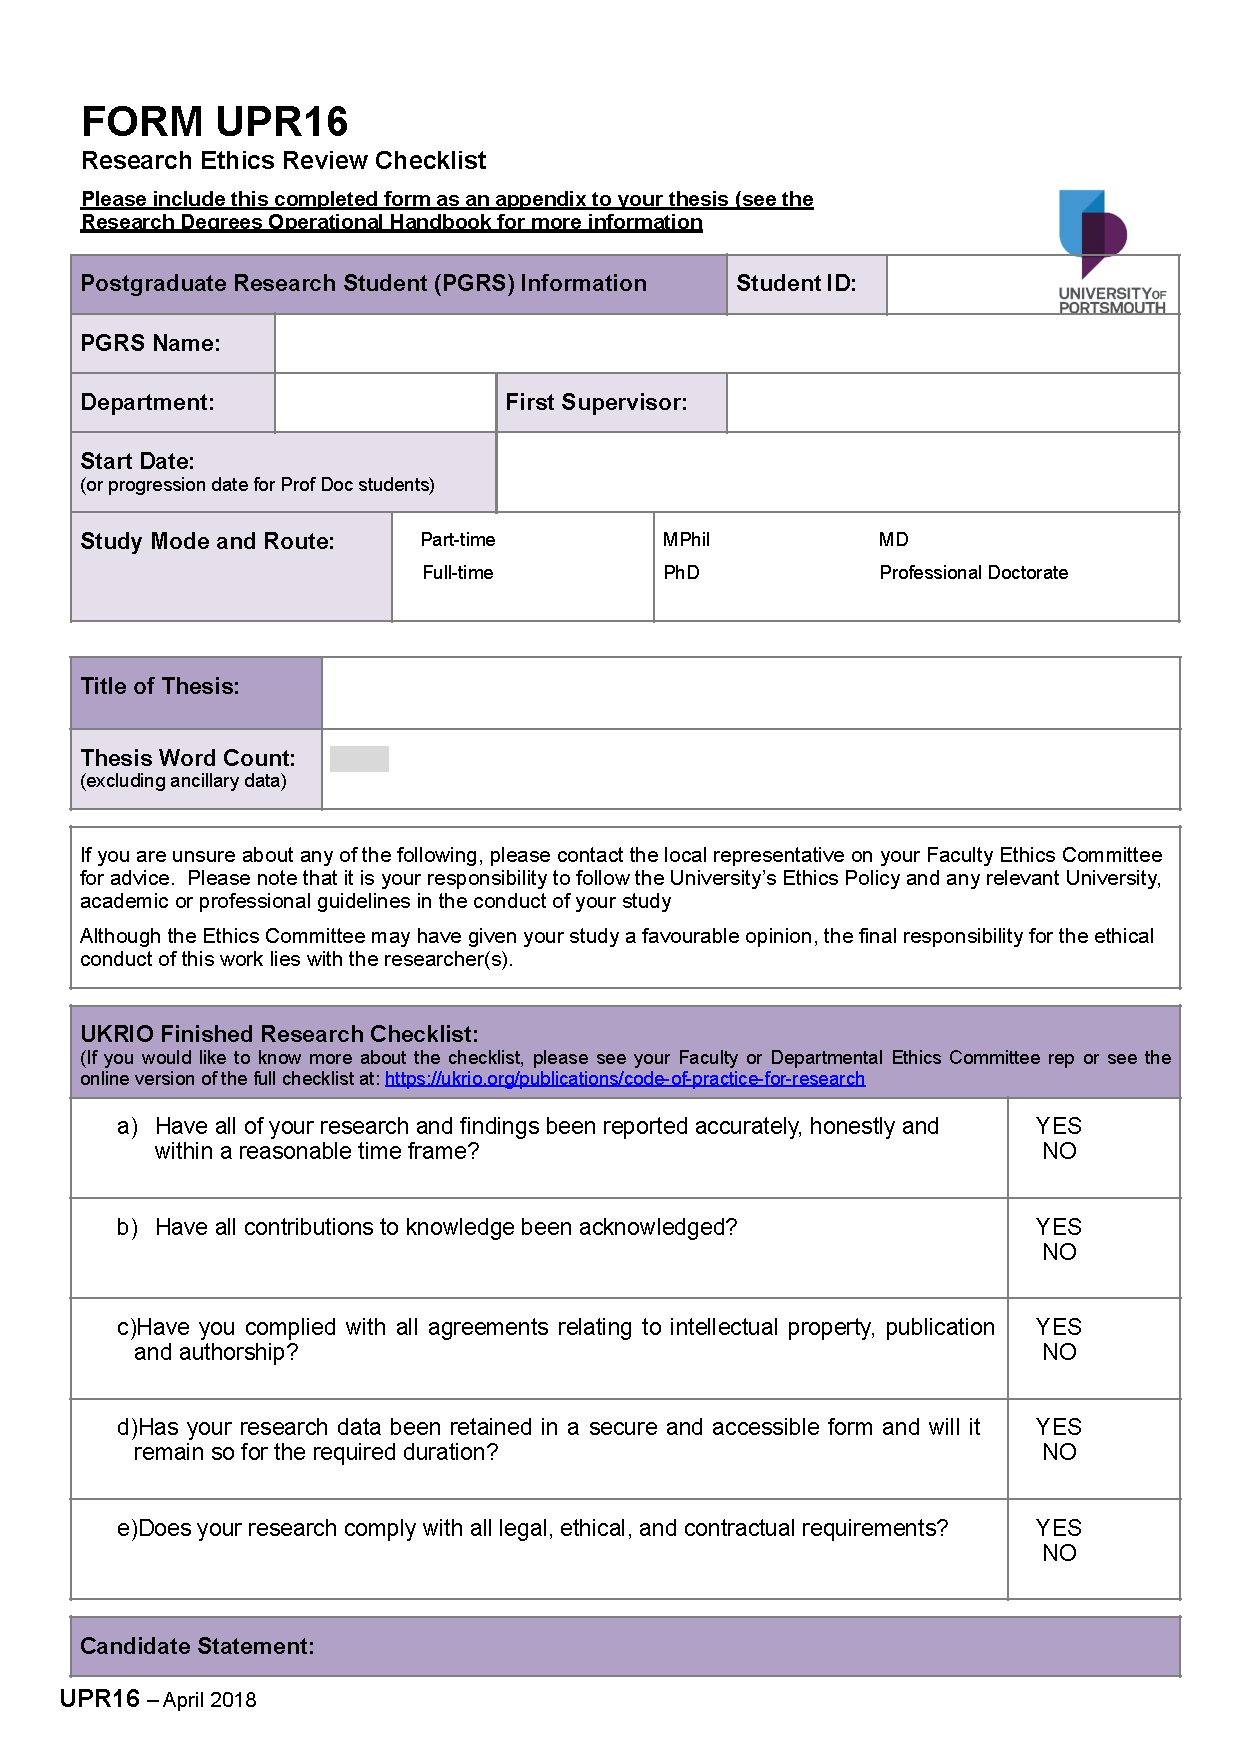
\includepdf[pages=-]{chapters/UPR16-Ethics-Review-Checklist.pdf} % Include the ethics form

\end{document}
